

\documentclass[../../e3_tp2_main.tex]{subfiles}

\begin{document}
\section{Ejercicio 5}

En esta secci\'on, el objetivo es estudiar el comportamiento de una compuerta \textit{or} CMOS y de una \textit{and} TTL, as\'i como la interacci\'on entre ambas. En particular haremos \'enfasis en qu\'e ocurre cuando una de las entradas est\'a flotante.\par


\subsection{Compuerta \textit{and} TTL}

Se utiliz\'o una de las 4 compuertas \textit{and} presentes en el integrado 74LS08, aliment\'andolo con $V_{CC} = 5V$. Para que esta alimentaci\'on fuese m\'as estable que la que proporcionan las fuentes del laboratorio de la universidad, se incluy\'o un capacitor de desacople de 100nF, conectado entre $V_{CC}$ y tierra, y posicionado lo m\'as cercano al integrado posible. Otra consideraci\'on que se tuvo para reducir el ruido fue conectar las entradas de las \textit{gates} no utilizadas a $V_{CC}$ a trav\'es de una resistencia de $1k\Omega$, a fin de evitar que la salida de las mismas oscile\footnote{Esta pr\'actica se recomienda en la nota de aplicaci\'on \href{https://www.fairchildsemi.com/application-notes/AN/AN-363.pdf}{\underline{\textit{Designing with TTL}} de \textit{Fairchild Semiconductors}} (consultado: 05/10/18).}.\par

La compuerta de inter\'es se conect\'o con una entrada al nivel alto, es decir a $V_{CC}$, tambi\'en pasando por una resistencia de $1k\Omega$.

\begin{figure}[H]
	\centering
	\begin{circuitikz}
		\draw
		(0,0) node[and port] (and){}
		(and.in 1) -| (-1.5,0.5) 
		to [R=1k$\Omega$] (-1.5, 2.3) node[ocirc, label=above:$V_{CC}$]{}
		(and.in 2) -| (-1.5,-0.27) node[ocirc, label=left:$V_{in}$]{}
		(and.out) -| (0.5,0)node[ocirc, label=right:$V_{out}$]{}	
	;\end{circuitikz}
	\caption{Conexi\'on de la compuerta TTL}
\end{figure}

De acuerdo a las propiedades del \'algebra de Boole, $x \cdot 1 = x$, y por lo tanto la salida deber\'ia estar en el mismo nivel l\'ogico que la entrada (lo cual se verific\'o experimentalmente). Se observ\'o que al dejar la entrada flotante, la salida se fijaba en el valor alto, midi\'endose a la salida aproximadamente $4.4V$. Realizando un DC \textit{sweep}, se determin\'o que esto implica que la tensi\'on flotante fue consistentemente mayor a $1.3V$, puesto que para tensiones menores la salida ser\'ia 0. 

\subsection{Compuerta \textit{or} CMOS}

El integrado utilizado fue el 74HC32. Al igual que para el LS, se aliment\'o con $V_{CC}=5V$, utilizando un capacitor de desacople de $100nF$. Las entradas de las compuertas no utilizadas, en cambio, se conectaron a tierra.\par

En este caso, se conect\'o una entrada a tierra y la otra se dej\'o flotante. An\'alogamente al caso anterior, como $x + 0 = x$, la salida deber\'ia ser igual a la entrada. Esto se pudo verificar cuando la entrada estaba fija en un valor, pero no as\'i para el caso que se quiere estudiar.\par

\begin{figure}[H]
	\centering
	\scalebox{1.2}{
	\begin{circuitikz}
		\draw
		(0,0) node[or port] (or){}
		(or.in 1) -| (-2,0.3) node[ocirc, label=left:$V_{in}$]{}
		(or.in 2) -| (-2,-0.27) node[ground]{}
		(or.out) -| (0.5,0)node[ocirc, label=right:$V_{out}$]{}	
	;\end{circuitikz}}
	\caption{Conexi\'on de la compuerta CMOS}
\end{figure}

Cuando la entrada no se fijaba en ning\'un valor, lo observado era lo siguiente: 

\begin{figure}[H]
	\centering
	\fbox{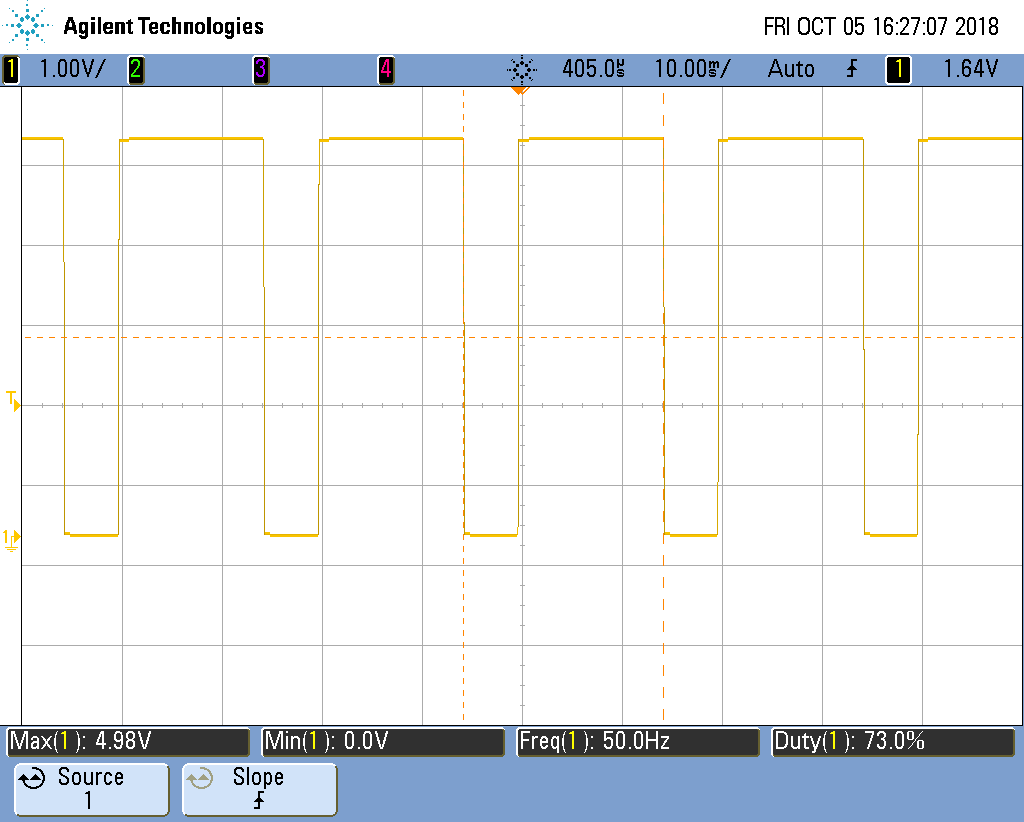
\includegraphics[scale=0.3]{../mediciones/e3_tp2_5_cmos1.png}}
	\caption{Salida del \textit{or} CMOS con una entrada flotante}
\end{figure}

Esta se\~nal cuadrada se debe a que la alta impedancia de la compuerta provoca que sea muy susceptible al ruido, y por lo tanto oscila con los $50Hz$ de la l\'inea. Cabe aclarar que esta oscilaci\'on no se observaba siempre: moviendo los cables y tocando las conexiones se pod\'ian obtener tanto ceros como unos l\'ogicos. \par

En cuanto al DC \textit{sweep}, en este caso indic\'o que la tensi\'on de entrada estaba oscilando entre tensiones menores y mayores a 2.2V, puesto que a partir de la misma la salida resultaba ser 1 y viceversa.


\subsection{Compuerta CMOS cargando a la compuerta TTL}

Habiendo estudiado el comportamiento de cada compuerta por separado, se procedi\'o a observar la interacci\'on entre ambas, conectando la salida del \textit{and} a la entrada del \textit{or}.

\begin{figure}[H]
	\centering
	\begin{circuitikz}
		\draw
		(0,0) node[and port] (and){}
		(2,-0.27) node[or port] (or){}		
		
		(and.in 1) -| (-1.5,0.5) to [R=1k$\Omega$] (-1.5, 2.3) node[ocirc, label=above:$V_{CC}$]{}
		(and.in 2) -| (-1.5,-0.27) node[ocirc, label=left:$V_{in}$]{}
		
		(and.out) to [short, -*] (or.in 1)
		(or.in 2) -| (0.2,-0.54) node[ground]{}
		(or.out) -| (2.5,-0.27) node[ocirc, label=right:$V_{out}$]{}			
	;\end{circuitikz}
	\caption{Conexi\'on entre las compuertas TTL y CMOS}
\end{figure}

Por lo discutido anteriormente, idealmente la salida de este circuito tiene el mismo valor l\'ogico que la entrada. Esto se verific\'o al fijar la tensi\'on de entrada en un valor determinado, consistentemente observando el mismo valor a la salida. Al dejar la entrada flotante, a la salida se observaba un 1 l\'ogico. Esto es consistente con lo obtenido para la TTL aislada, puesto que si su salida cuando la entrada es flotante es 1, tambi\'en lo ser\'a la salida de todo el circuito.\par

El DC \textit{sweep} de esta configuraci\'on est\'a tambi\'en en l\'inea con lo analizado hasta el momento. Si bien el valor de $V_{in}$ para el cual la salida transiciona de 0 a 1 no es exactamente igual a los $1.3V$ que se obtuvieron para la TTL, si no que fue de $1.4V$, la diferencia entre ambos es de un $7\%$, lo cual est\'a dentro de un rango razonable.

\begin{figure}[H]
	\centering
	\fbox{\includegraphics[scale=0.3]{../mediciones/e3_tp2_5_1.png}}
	\caption{DC \textit{sweep} del circuito TTL-CMOS}
\end{figure}



\subsection{Conclusiones}

De acuerdo a los resultados obtenidos, las compuertas CMOS son m\'as susceptibles al ruido que las TTL si se las deja flotantes. De no fijar la entrada de una CMOS, es probable que se induzca ruido proveniente de la linea. Si bien esto no se observ\'o en la TTL, es una buena pr\'actica fijar entradas no utilizadas a un valor l\'ogico determinado, de acuerdo a la bibliograf\'ia consultada.


\end{document}
